%%%%%%%%%%%%%%%%%%%%%%%%%%%%%%%%%%%%%%%%%
%\title{Title page with logo}
%----------------------------------------------------------------------------------------
%	PACKAGES AND OTHER DOCUMENT CONFIGURATIONS
%----------------------------------------------------------------------------------------

\documentclass[12pt]{article}
\usepackage[english]{babel}
\usepackage[utf8x]{inputenc}
\usepackage{amsmath}
\usepackage{graphicx}
\usepackage[colorinlistoftodos]{todonotes}
\usepackage{float}
\usepackage[export]{adjustbox}
\usepackage{wrapfig}

\begin{document}

\begin{titlepage}

\newcommand{\HRule}{\rule{\linewidth}{0.5mm}} % Defines a new command for the horizontal lines, change thickness here

\center % Center everything on the page
 
%----------------------------------------------------------------------------------------
%	HEADING SECTIONS
%----------------------------------------------------------------------------------------

\textsc{\LARGE Università degli studi di Milano Bicocca}\\[1.5cm] % Name of your university/college
\textsc{\Large Gruppo-BrewDay-2}\\[0.5cm] % Major heading such as course name
\textsc{\large Progetto-BrewDay-2}\\[0.5cm] % Minor heading such as course title

%----------------------------------------------------------------------------------------
%	TITLE SECTION
%----------------------------------------------------------------------------------------

\HRule \\[0.4cm]
{ \huge \bfseries Brew Day!}\\[0.4cm] % Title of your document
\HRule \\[1.5cm]
 
%----------------------------------------------------------------------------------------
%	AUTHOR SECTION
%----------------------------------------------------------------------------------------

\begin{minipage}{0.45\textwidth}
\begin{flushleft} \large
\emph{Author:}\\
David \textsc{Chieregato} 806961 % Your name
Davide \textsc{Ditolve} 806953
\end{flushleft}
\end{minipage}
~
\begin{minipage}{0.45\textwidth}
\begin{flushright} \large
~\newline
Chunhua \textsc{He} 804350\\
Luca \textsc{De Filippi} 757401\\
\end{flushright}
\end{minipage}\\[2cm]

% If you don't want a supervisor, uncomment the two lines below and remove the section above
%\Large \emph{Author:}\\
%John \textsc{Smith}\\[3cm] % Your name
%----------------------------------------------------------------------------------------
%	LOGO SECTION
%----------------------------------------------------------------------------------------


\includegraphics[width=0.3\textwidth]{logo.jpg}\\% Include a department/university logo - this will require the graphicx package
 
%----------------------------------------------------------------------------------------

\vfill % Fill the rest of the page with whitespace

\end{titlepage}


\begin{abstract}
Home brewing, the process of producing beer on a small scale for personal purposes, is an activity that receives growing attention among beer enthusiasts. Every home brewer owns a brewing equipment (kettles, fermenters, pipes, etc.) with a certain maximum brewing capacity, the number of litres the equipment is able to handle in a single "batch". Brewing also requires ingredients, whose actual amounts vary from recipe to recipe; these are various kinds of malts, hops, yeasts and sugars (and of course, water). Brewers like to log their recipes, for future reference, and maintain an updated list of available ingredients, for shopping before the next brew.

The goal of this project is to develop an application for home brewers thats allows them to maintain a list of recipes, and adapt existing ones. The application must also maintain a list of available ingredients, update this list after a batch and when new ingredients are bought, and produce shopping lists for the next batch. A special characteristic of the application is the "what should I brew today?" feature: it goes through the recipes, and taking into account the available ingredients and brewing capacity of the equipment selects a recipe that can be brewed with the available ingredients, maximizing the use of the ingredients, and the batch size.
Brew Day! is an application that allows home brewers to maintain an organized database of their beer recipes. The application allows users to create, store and modify recipes, and later on delete them, if the user wishes to do so. The application is intended for "all-grain" brewers only, and thus all recipes are for this kind of brews (the "extract" brews are not supported).

Every home brewer has a specific equipment, whose characteristics leads to a particular "batch size", the maximum number of litres that can be brewed on a single run. Recipes involve, besides water:
malts
hops
yeasts
sugars
additives
While brewers prefer to create recipes referring to concrete values, like kilograms of a specific malt or grams of a specific hops, the application must store these recipes in some "absolute" measure, that allows for a direct conversion of the recipe when the equipment, and consequently the batch size, is updated. For instance, expressing malt quantities as a percentage of the total, and hops as grams per litre of mash, is a possibility.

Besides the actual recipes, the application must maintain recipe instances, i.e., particular brews based on a recipe; these instances can be accompanied by notes to refer to issues that may affect the resulting beer and the brewers would like to keep logged. A particular kind of note is the tasting notes, that allows brewers to keep track of opinions on a beer from a particular brew.

Besides these more traditional features of Brew Day!, the application maintains a list of available ingredients. This allows brewers to be notified about missing ingredients for the next brew. A recipe instance, i.e., a particular brew, should allow users to update the available ingredients list, substracting used ingredients from the available ones. Related to this information, Brew Day! must support a useful feature for brewers: "what should I brew today?" goes through the recipes database, and chooses the recipe that maximizes the use of the available ingredients, taking into account the equipment capacity, of course.

The project must implement the features described above, i.e., creation, modification and deletion of recipes, creation of recipe instances (brews), support for notes on brews, and keeping track of available ingredients. The "what should I brew today?" is a mandatory feature. Optionally, developers may choose to allow ingredients availability manually, as opposed to do it automatically from brews information.

The choice of the development platform, including tools and programming languages to use, is left to the teams. The application may be desktop-based, web-based or even tailored for portable devices. Besides the development of the software, teams must provide accompanying documentation, including a requirements document, a design document, and a brief user manual (installation and usage of the application).

\end{abstract}
\vfill
\section{Assunzioni e glossario}
\section{Requirements}

The goal of this project is to develop an application for home brewers thats allows them to mantain a list of recipes, and adapt esisting ones.
This application is intended for the "all-grain" users only, thus "extract" brews are not supported. \\
\\
Functional Requirements:\\
\\
User's account:
\begin{itemize}
\item The application allows users to create an account

\item The application allows users to login in their account

\item Every user have specific equipment which can produce a maximum "batch size"\\
\end{itemize}
User's recipe:
\begin{itemize}
\item The application allows users to create a recipe

\item The application allows users to store a recipe 

\item The application allows users to update a recipe

\item The application allows users to delete a recipe

\item The application stores recipe's ingredients in an "absolute" measure; eg. total percentage

\item Recipes are made by ingredients: Water, Malts, Hops, Yeasts, Sugars, Additives
\end{itemize}
\newpage
Recipes ingredients:\\
\begin{itemize}
\item The application mantain a list of available ingredients

\item The application notifies users about missing ingredients

\item The application update ingredients's list after a batch

\item The application update ingredients's list when new ingredients are bought

\item The application produce a shopping list for the next batch \\
\end{itemize}
Additional features:
\begin{itemize}
\item The application supports notes for brews

\item The application has "what should i brew today" feature:

\item With the "what should i brew today" feature, the application suggest a recipe made with the available ingredients.

\item With the "what should i brew today" feature, the suggested recipe maximizes the usage of available ingredients.

\item With the "what should i brew today" feature, the suggested recipe maximizes the batch size.
\end{itemize}

\section{Use Case}
\subsection{Use Case Diagram}
\begin{figure}[H]
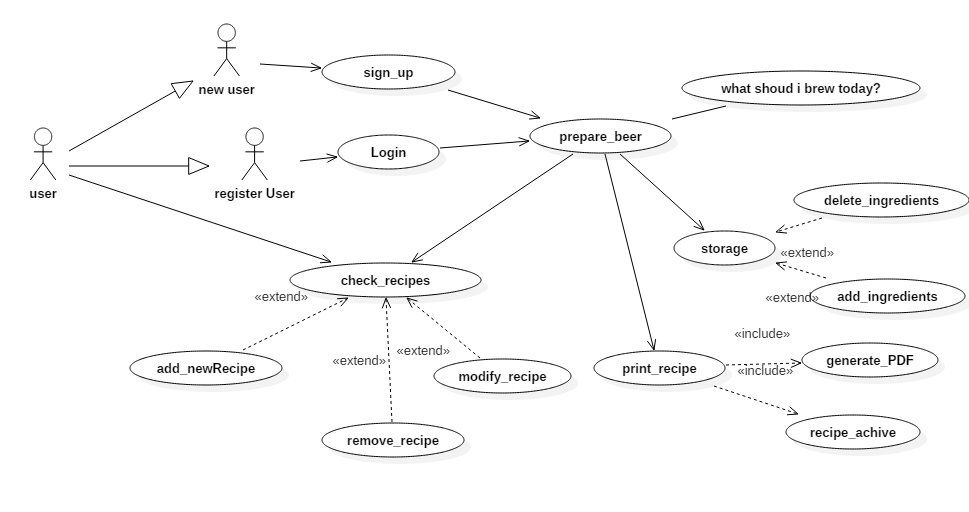
\includegraphics[scale=0.8]{UseCaseDiagram.png}
\centering
\end{figure}
\subsection{Use Case Description}
\begin{itshape}
What Should I Brew Today?
\end{itshape}\\
Portata: Web Page\\
Livello: Obiettivo Utente\\
Attore Primario: Utente che desidera creare un tipo di birra\\
Parti Interessate e Interessi: Sistema\\
Pre-condizioni: Log-In\\
Garanzia di successo: Presenza ingredienti nel magazzino\\
Scenario Principale di Successo:
\begin{enumerate}
\item Utente seleziona il "catalogo"
\item Utente seleziona ingrediente
\item Utente accede al catalogo-ricetta
\item Sistema mostra l'elemento selezionato
\end{enumerate}
Scenari alternativi:\\
Fallimento: il sistema comunica l'errore o "elemento non trovato"\\
Requisiti speciali: Nessuno\\
Elenco delle variabili tecnologiche e dei dati: Nessuna\\
Frequenza di ripetizione: Nessuna
\bigskip
\\
\begin{itshape}
Sign-Up
\end{itshape}\\
Attore Primario: Utente che desidera registrarsi\\
Parti Interessate: Utente, Sistema\\
Scenario Principale di Successo:
\begin{enumerate}
\item Utente fornisce un indirizzo email
\item Utente fornisce un nickname
\item Utente fornisce una password
\item Utente si registra con successo
\end{enumerate}
Scenari alternativi:\\
Fallimento: Sistema invia un messaggio per invitare utente a riprovare
\begin{enumerate}
\item Email già registrata
\item Nickname invalido oppure già presente
\item Password non risponde ai criteri stabiliti dal sistema
\end{enumerate}
\bigskip
\begin{itshape}
Sign-In
\end{itshape}\\
Attore Primario: Utente che desidera accedere all'applicazione\\
Parti Interessate: Utente, Sistema\\
Scenario Principale di Successo:\\
\begin{enumerate}
\item Utente immette email e password
\item Uente accede all'applicazione
\end{enumerate}
Scenari Alternativi:\\
Fallimento: Sistema invita a riprovare ad effettuare il log-in
\bigskip
\\
\begin{itshape}
Check-Recipe
\end{itshape}\\
Attore Primario: Utente che desidera consultare le ricette\\
Parti Interessate: Utente, Sistema\\
Scenario Principale: Utente accede al catalogo delle ricette
\bigskip
\\
\begin{itshape}
Add-New-Recipe
\end{itshape}\\
Attore Primario: Utente desidera aggiungere la propria ricetta al catalogo\\
Parti Interessate: Utente, Sistema\\
Scenario Principale: Utente crea una nuova ricetta\\
Scenari Alternativi:\\
Fallimento: Utente non fornisce una composizione valida
\bigskip
\\
\begin{itshape}
Modify-Recipe
\end{itshape}\\
Attore Primario: Utente desidera apportare modifiche a ricette nel catalogo\\
Parti Interessate: Utente, Sistema\\
Scenario Principale: 
\begin{enumerate}
\item Utente modifica uno o più ingrediente presenti in una ricetta
\item Utente modifica la quantità di uno o più ingrediente della ricetta
\item Utente apporta le modifiche
\end{enumerate}
Scenari Alternativi:\\
Fallimento: Utente apporta modifiche non valide
\bigskip
\\
\begin{itshape}
Delete-Recipe
\end{itshape}\\
Attore Primario: Utente che desidera cancellare ricette presenti nel ricettario\\
Parti Interessate: Utente, Sistema\\
Scenario Principale: Utente cancella la ricetta
\bigskip
\\
\begin{itshape}
Add-Ingredient
\end{itshape}\\
Attore Primario: Utente che aggiunge nuovi ingredienti nel magazzino\\
Parti Interessate: Utente, Sistema\\
Scenario Principale: \\
\begin{enumerate}
\item Utente inserisce ingrediente
\item Sistema controlla se ingrediente è presente in magazzino
\item Sistema inserisce ingrediente nel database
\end{enumerate}
Scenari Alternativi:\\
Fallimento: Sistema informa utente che ingrediente è già presente nel magazzino\\
\begin{enumerate}
\item Ingrediente già presente nel database
\end{enumerate}
\bigskip
\begin{itshape}
Delete-Ingredient
\end{itshape}\\
Attore Primario: Utente che desidera cancellare ingredienti dal magazzino\\
Parti Interessate: Utente, Sistema\\
Scenario Principale: Sistema cancella ingrediente selezionato dall'utente
\bigskip
\\
\begin{itshape}
Prepare-Beer
\end{itshape}\\
Attore Primario: Utente che desidera preparare una birra\\ 
Parti Interessate: Utente, Sistema\\
Scenario Principale:
\begin{enumerate}
\item Utente accede alla sezione ricettario
\item Utente inserisce gli ingredienti disponibili
\item Sistema visualizza le possibili ricette che si possono creare
\item Sistema visualizza gli ingredienti mancanti
\item Sistema visualizza gli strumenti necessari per preparare la ricetta
\end{enumerate}
\pagebreak
\section{Activity}
We decided to focus on the most complex function to be showed in this Activity Diagram: What Should I Brew Today?\\
\begin{figure}[H]
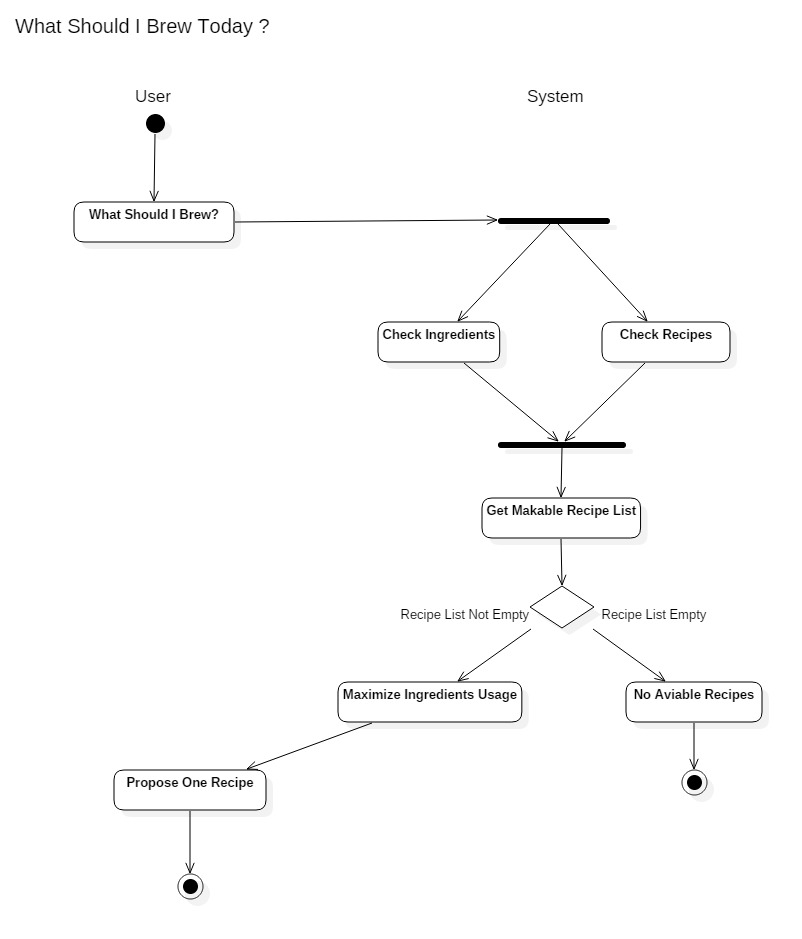
\includegraphics[scale=0.49]{ActivityDiagram.jpg}
\centering
\end{figure}
\pagebreak
\section{Sequence}
\begin{figure}[H]
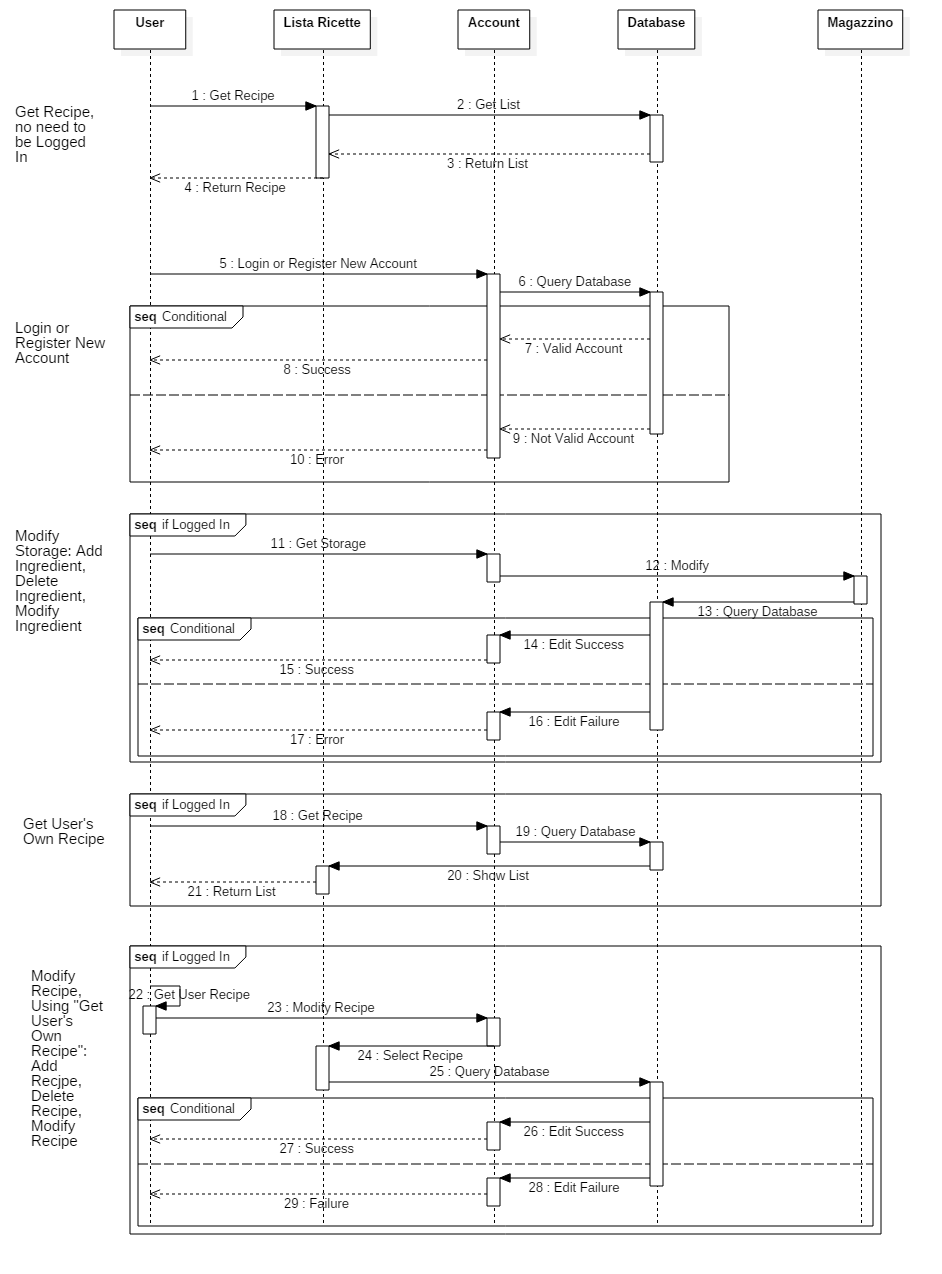
\includegraphics[scale=0.5]{SequenceDiagram1.png}
\centering
\end{figure}
\thispagestyle{empty}
\pagebreak
In these Sequence Diagrams is evidenced the flow of information from one actor to another.\\
To be noticed that every action made by the User is always filtered by a view, Lista Ricette or Account, which makes the actual query to the needed database.\\
\section{Domain}
The following diagram express a view of the BrewDay! internal structure and hierarchy.\\
On this diagram is evidenced the needed information to log in and the dual nature of the Recipes class: Public and Private, which is defined by a boolean attribute.
\begin{figure}[H]
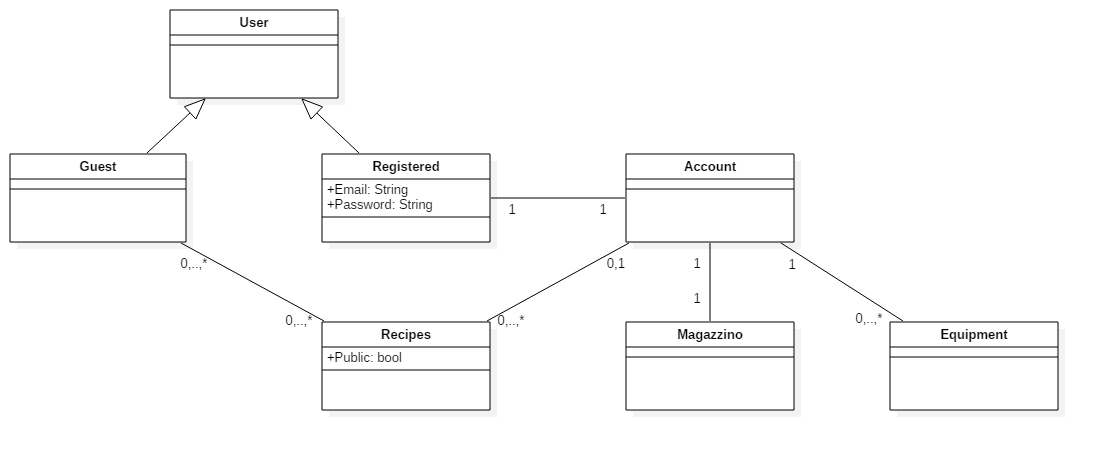
\includegraphics[width=1.25\textwidth, left]{DomainDiagram.jpg}
\end{figure}

\pagebreak
\section{Statechart}
The following diagram shows the operations that can be made in every state.\\
Each one of this States represent a view.
\begin{figure}[H]
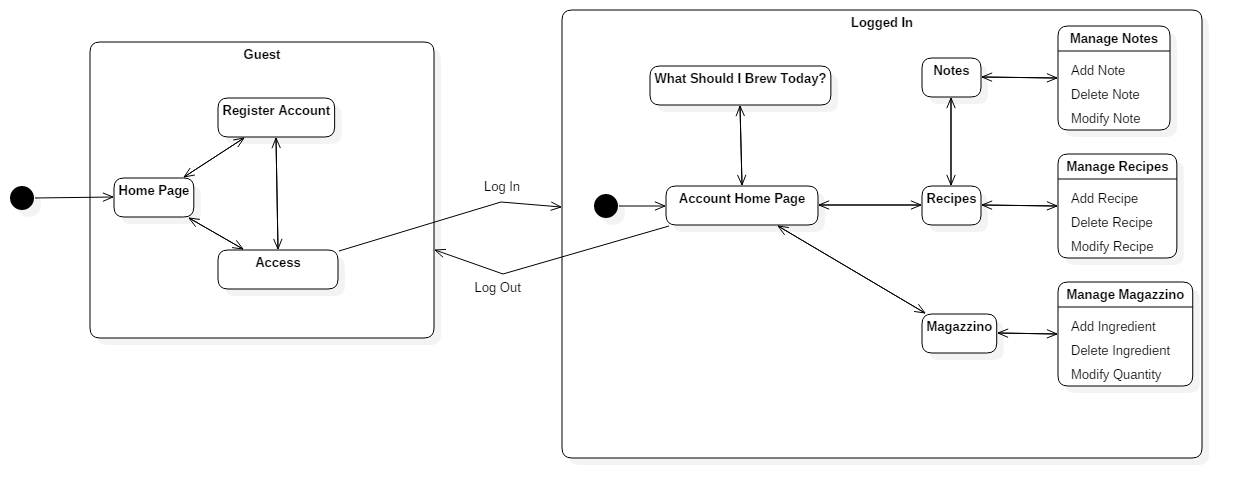
\includegraphics[scale=0.4]{Statechart.png}
\end{figure}
\section{Implementation Choices}
\subsection{DAO Pattern}
In web programming, the Data Access Object Pattern is an Architectural Pattern used to manage Persistence:\\
it's a class with its methods that represents a table entity of a Relational Database Management System.\\
Mainly used to stratify and isolate the access to a table by queries, placed in class methods, hence creating a separation from data layer to business logic and making the code more abstract and maintainable.\\
\\
\begin{itshape}
Advantages:
\end{itshape}
\begin{itemize}
\item Makes a rigid separation from application components, like 
\begin{itshape} 
Model 
\end{itshape} and 
\begin{itshape}
Control
\end{itshape} of a MVC based application
\end{itemize}
\subsection{MVC Pattern}
MVC Pattern stands for Model-View-Controller Pattern. It's an Architectural Pattern made by three sections.\\
The Model catch the application behavior, directly handling data, logic and application's rules.\\
A View is every output representation of information.\\
The Controller accept a input and translate in commands for the model or the view.\\
\section{Classes}
\section{Test}
\subsection{SonarQube}

After a first execution of the SonarQube test engine we noticed that the worst code quality issue where related to Jquery javascript plugin.\\
Jquery is a rewrite engine, so it's normal that the code quality analysis result is not good: it's creating a different way
to use the javascript language so it needs a different kind of language test.
\begin{figure}[H]
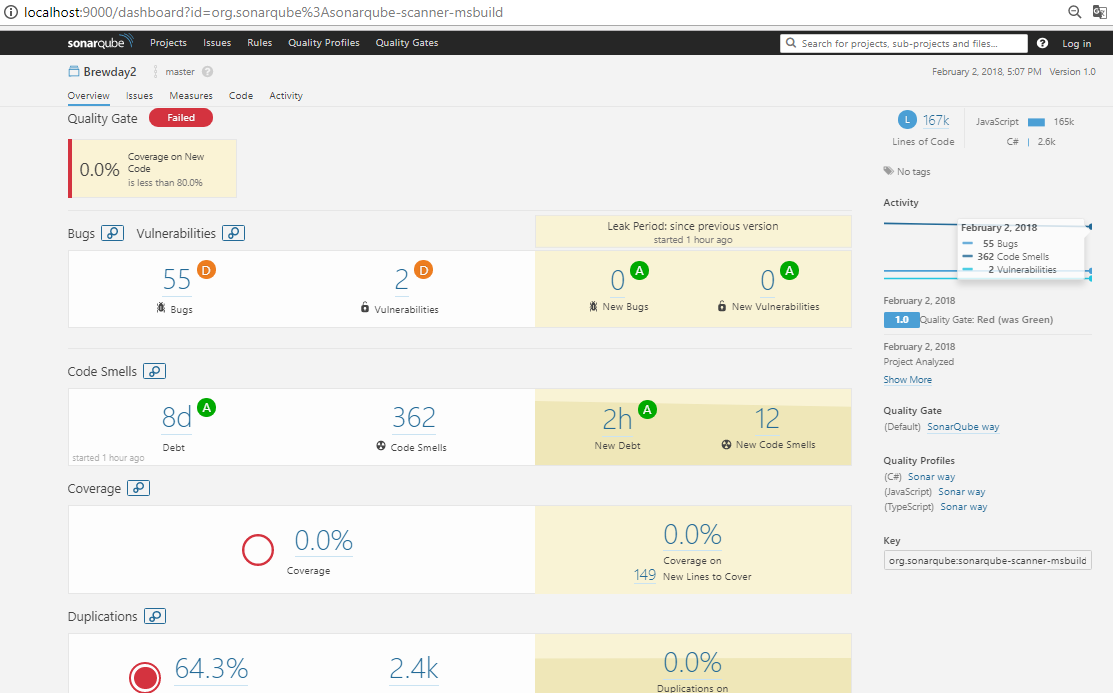
\includegraphics[scale=0.5]{sonar1.png}
\end{figure}
\pagebreak
So we concentrated on the C\# issues exposed by SonarQube.
\begin{figure}[H]
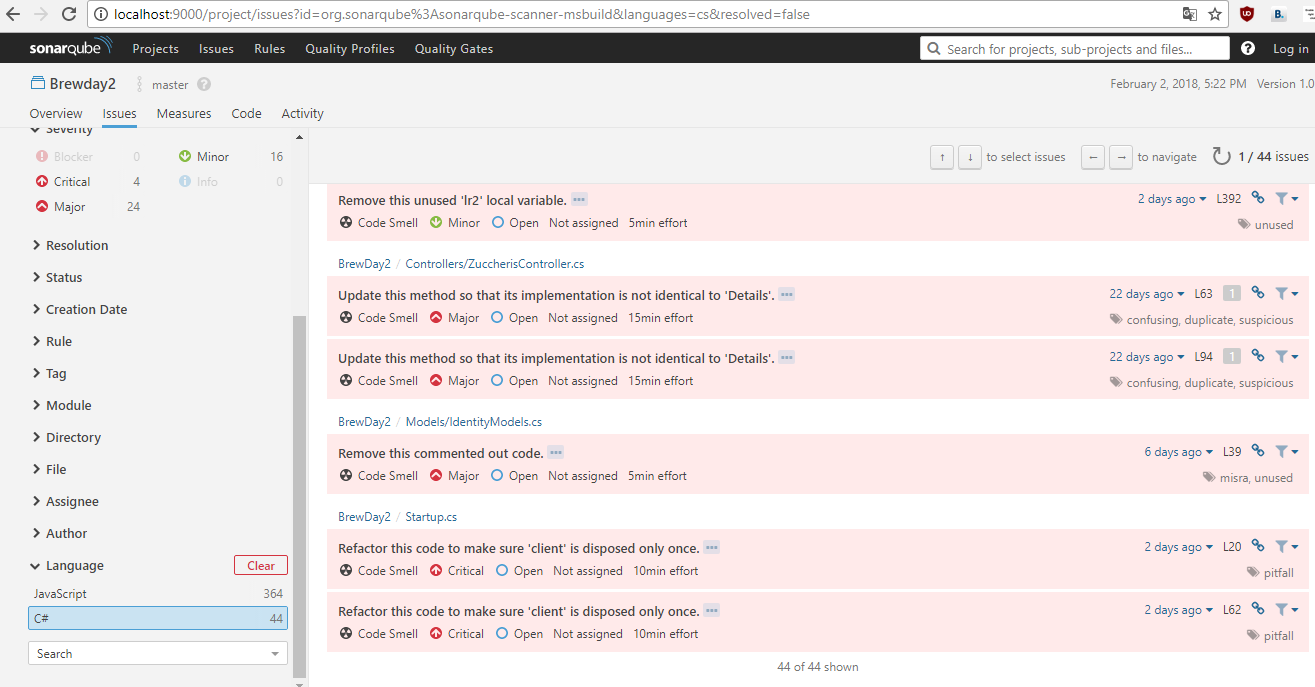
\includegraphics[scale=0.5]{sonar2.png}
\end{figure}
\pagebreak
After excluding JS related libraries from the analysis we removed the worst issues and the code quality now gets an 'A'.
\begin{figure}[H]
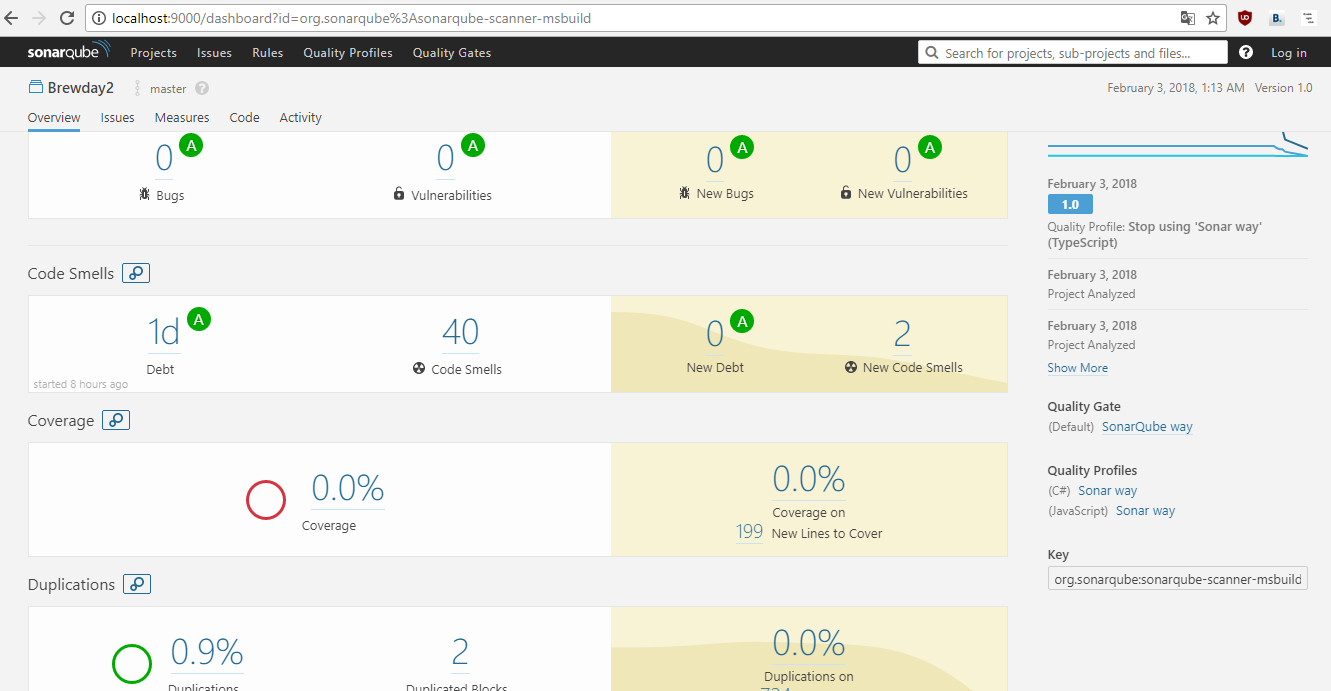
\includegraphics[scale=0.5]{sonar3.png}
\end{figure}
\pagebreak
We managed to fix almost all the code-smells detected:
\begin{figure}[H]
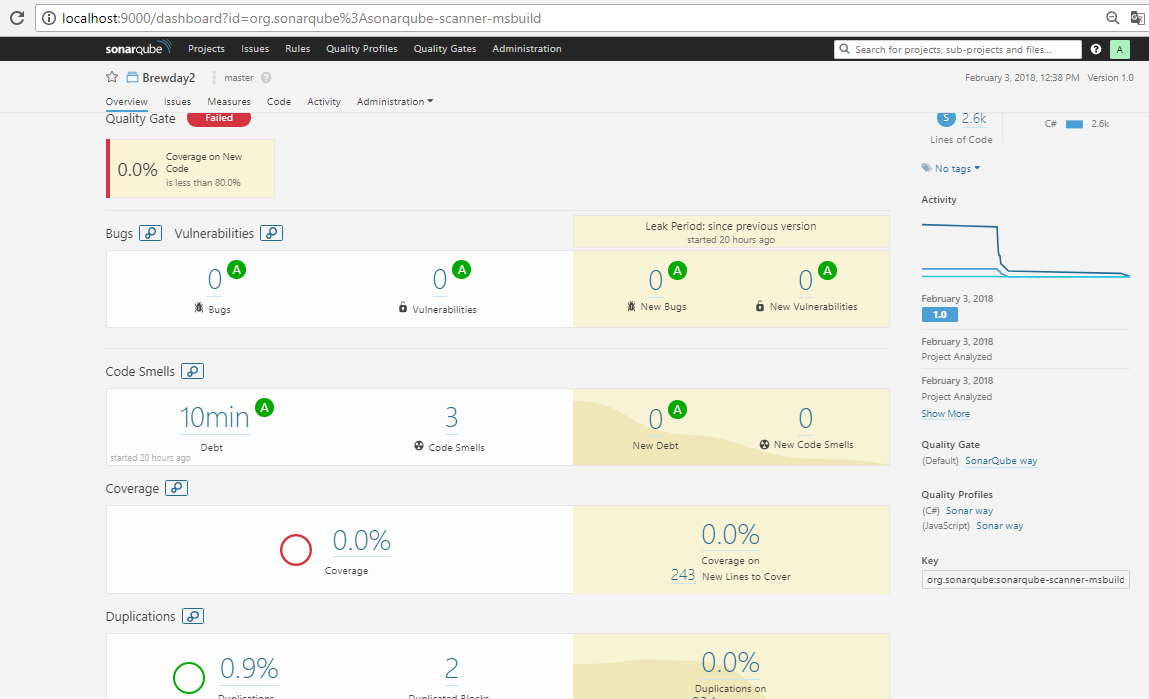
\includegraphics[scale=0.5]{sonar4.png}
\end{figure}
\pagebreak
Only a few complexity related issue are still not addressed, one is related to the "What should I brew Today" feature that needs a lot of data computation to be executed and it wouldn't be a good choice to divide it in smaller functions because
there is no logical cohesion between sub-operations.\\
The other one is related to a C\# default account management function not written by us.
\begin{figure}[H]
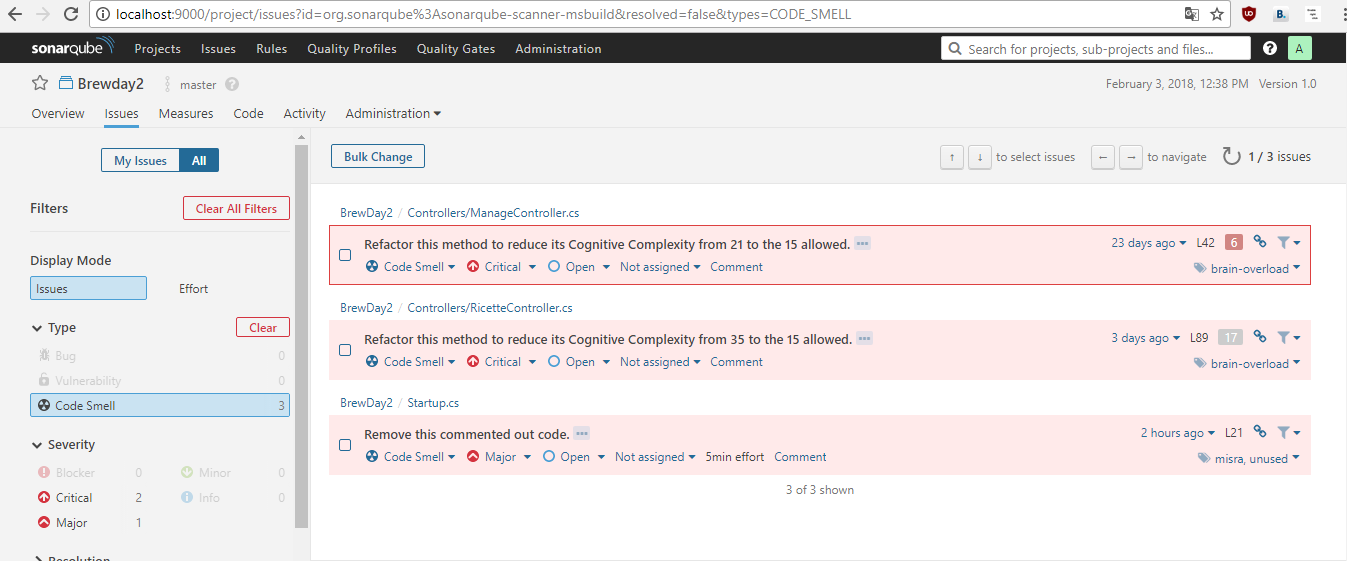
\includegraphics[scale=0.5]{code-smell.png}
\end{figure}
\subsection{Unit Test}
On the unit test side we did a lot of experimentations to make it available in the 
SonarQube report: MSTest, MSTest V2, Moq, AutoMoq, SimpleStubs, Nsubstitute, Rhino Mocks, nUnit and xUnit.\\
\linebreak
We tried every possible easily available option in order to get the code coverage working in SonarQube, but it seems that it doesn't support most of the standard C\# testing frameworks available in Visual Studio.\\
\linebreak
The only one that seems to be supported is OpenCover, however it's very complicated to set-up (tricky configuration) and it's not issue-free as we can see from
their github https://github.com/OpenCover/opencover/issues/121 (they are passing the buck to SonarQube).\\
\linebreak
So we decided to implement our tests in the standard Visual Studio MSTest V2 platform.\\
The tests cover most of the code, but it won't be visible in the SonarQube report.\\
Every controller has from one to five tests per Method in order to make sure everything is working.

\end{document}
